\begin{theorem} (О замене переменной в гладкой дифформе)
	Если $V \subset \R^m$, $U \subset \R^n$ --- области, $\phi \colon V \to U$ --- диффеоморфизм и $\Omega$ --- гладкая $p$-форма на $U$, имеющая такой вид:
	\[
		\Omega(x) = w_{i_1, \ldots, i_p}(x) dx^{i_1} \wedge \ldots \wedge dx^{i_p}
	\]
	где суммирование идёт по наборам $1 \le i_1 < \ldots < i_p \le n$. Тогда для дифформы $\phi^*\Omega$ верна формула:
	\[
		\phi^*\Omega(y) = w_{i_1, \ldots, i_p}(\phi(y))d\phi^{i_1}(y) \wedge \ldots \wedge d\phi^{i_p}(y)
	\]
\end{theorem}

\begin{proof}
	Дифформы совпадают, если их значения одинаковы на всех базисных наборах. Пусть $G = (g_1, \ldots, g_m)$ --- базис $\R^m$. Распишем значение на левой дифформе:
	\begin{multline*}
		\phi^*\Omega(y)(g_{k_1}, \ldots, g_{k_p}) = \Omega(\phi(y))(\phi'(y)(g_{k_1}), \ldots, \phi'(y)(g_{k_p})) =
		\\
		w_{i_1, \ldots, i_p}(\phi(y)) dx^{i_1} \wedge \ldots \wedge dx^{i_p}(\phi'(y)(g_{k_1}), \ldots, \phi'(y)(g_{k_p})) =
		\\
		w_{i_1, \ldots, i_p}(\phi(y)) \det(dx^{i_j}(\phi'(y)(g_{k_l})))
	\end{multline*}
	Теперь сделаем подстановку в правую дифформу:
	\[
		w_{i_1, \ldots, i_p}(\phi(y))d\phi^{i_1}(y) \wedge \ldots \wedge d\phi^{i_p}(y)(g_{k_1}, \ldots, g_{k_p}) = w_{i_1, \ldots, i_p}(\phi(y)) \det(d\phi^{i_j}(y)(g_{k_l}))
	\]
	Если установить равенство между элементами детерминантов, то требуемое будет доказано. А это уже объяснялось в примере выше.
\end{proof}

\begin{corollary}
	Если $V \subset \R^m$, $U \subset \R^n$ --- области, $\phi \colon V \to U$ --- диффеоморфизм и $\Omega$ --- гладкая $p$-форма на $U$, то имеет место равенство:
	\[
		d(\phi^*\Omega) = \phi^*d\Omega
	\]
\end{corollary}

\begin{proof}~
	\begin{enumerate}
		\item $p = 0$. Тогда дифференциальная форма вырождается в обычную функцию. Приведём по-отдельности левую и правую часть к одинаковой форме:
		\[
			d(\phi^*\Omega(y)) = d(\Omega(\phi(y))) = \pd{\Omega}{x_i}(\phi(y)) d\phi^i(y)
		\]
		Теперь для правой части:
		\[
			\phi^*d\Omega(y) = \phi^*\ps{\pd{\Omega}{x_i}(\cdot)dx^i}(y) = \pd{\Omega}{x_i}(\phi(y)) d\phi^i(y)
		\]
		
		\item $p \ge 1$. Пусть форма $\Omega$ записана в такой форме:
		\[
			\Omega(x) = w_{i_1, \ldots, i_p}(x) dx^{i_1} \wedge \ldots \wedge dx^{i_p}
		\]
		По теореме о замене переменной в гладкой дифформе можем записать следующее:
		\begin{multline*}
			d\phi^*\Omega(y) = d(w_{i_1, \ldots, i_p}(\phi(y))d\phi^{i_1}(y) \wedge \ldots \wedge d\phi^{i_p}(y)) =
			\\
			dw_{i_1, \ldots, i_p}(\phi(y)) \wedge d\phi^{i_1}(y) \wedge \ldots \wedge d\phi^{i_p}(y) + w(\phi(y))d(d\phi^{i_1}(y) \wedge \ldots \wedge d\phi^{i_p}(y))
		\end{multline*}
		Дифференциал во втором слагаемом равен нулю по свойству дважды дифференцируемой дифформы, а потому остаётся расписать лишь первое слагаемое:
		\[
			d\phi^*\Omega(y) = \pd{w_{i_1, \ldots, i_p}}{x_j} (\phi(y)) d\phi^j(y) \wedge d\phi^{i_1}(y) \wedge \ldots \wedge d\phi^{i_p}(y)
		\]
		Теперь покажем, что для правой части исходного равенства получится аналогичная формула:
		\begin{multline*}
			\phi^*d\Omega(y) = \phi^*(dw_{i_1, \ldots, i_p}(x) \wedge dx^{i_1} \wedge \ldots \wedge dx^{i_p})(y) =
			\\
			\phi^*\ps{\pd{w_{i_1, \ldots, i_p}}{x_j}(x) dx^j \wedge dx^{i_1} \wedge \ldots \wedge dx^{i_p}}(y) =
			\\
			\pd{w_{i_1, \ldots, i_p}}{x_j}(\phi(y)) d\phi^j(y) \wedge d\phi^{i_1}(y) \wedge \ldots \wedge d\phi^{i_p}(y)
		\end{multline*}
	\end{enumerate}
\end{proof}

\begin{definition}
	Дифференцируемая $p$-форма $\Omega$ называется \textit{замкнутой в $U$}, если верно условие:
	\[
		\forall x \in U\ \ d\Omega(x) = 0
	\]
\end{definition}

\begin{definition}
	$p$-форма $\Omega$ называется \textit{точной в $U$}, если существует $(p - 1)$-форма $\Pi$ такая, что $\Omega = d\Pi$.
\end{definition}

\begin{note}
	Если в рамках предыдущего определения оказалось, что $\Pi$ дважды дифференцируема, то $d\Omega = d(d\Pi) = 0$, то есть $\Omega$ не только точна, но и замкнута.
\end{note}

\begin{definition}
	Отображение $\phi \colon \R^n \times [0; 1] \to \R^n$, заданное для $x_0 \in \R^n$ следующим образом:
	\[
		\phi(x, t) = x_0 + (1 - t)(x - x_0)
	\]
	называется \textit{прямым стягиванием}.
\end{definition}

\begin{definition}
	Область $U \subset \R^n$ называется \textit{звёздной относительно точки $x_0 \in U$}, если она допускает прямое стягивание в эту точку, то есть $\phi$ может рассматриваться как $\phi \colon U \times [0; 1] \to U$.
\end{definition}

\begin{center}
	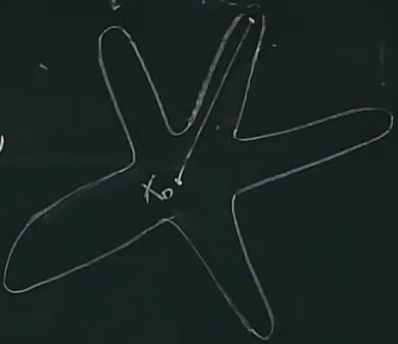
\includegraphics[width=0.4\textwidth]{images/star.png}
\end{center}

\begin{definition}
	Область $U \subset \R^n$ называется \textit{звёздообразной}, если она является диффеоморфным образом звёздной области.
\end{definition}

\begin{note}
	Рассмотрим $p$-форму $\Omega$ на $U \times [0; 1]$, где $U \subset \R^n$ (и область, естественно). Тогда при расписывании её по базису мы будем считать каноничными такие базисные формы:
	\begin{align*}
		&{a(x, t)dt \wedge dx^{i_1} \wedge \ldots \wedge dx^{i_{p - 1}},\ \ 1 \le i_1 < \ldots < i_{p - 1} \le n}
		\\
		&{b(x, t)dx^{i_1} \wedge \ldots \wedge dx^{i_p},\ \ 1 \le i_1 < \ldots < i_p \le n}
	\end{align*}
	Под \textit{сужением формы $\Omega$ на $U \times \{t_0\}$} мы будем понимать $p$-форму $\Omega|_{U \times \{t_0\}}$, полученную подстановкой $t = t_0$ в $\Omega$ и в которой занулили слагаемые с $dt$ (как будто бы в исходную форму стали приходить только вектора $U \times \{0\}$ и $dt$ потеряло смысл):
	\begin{align*}
		&{a(x, t)dt \wedge dx^{i_1} \wedge \ldots \wedge dx^{i_{p - 1}}|_{U \times \{t_0\}} = 0}
		\\
		&{b(x, t)dx^{i_1} \wedge \ldots \wedge dx^{i_p}|_{U \times \{t_0\}} = b(x, t_0)dx^{i_1} \wedge \ldots \wedge dx^{i_p}}
	\end{align*}
\end{note}

\textcolor{red}{Здесь можно было бы сделать картинку с типа плоскостями $U \times \{0\}$ и $U \times \{1\}$}

\begin{lemma}
	Пусть $\Omega$ --- гладкая $p$-форма на $U \times [0; 1]$, а $K$ --- линейное отображение на дифформах, заданное на базисных формах с функциональной координатой следующим образом:
	\begin{align*}
		&{K(a(x, t)dt \wedge dx^{i_1} \wedge \ldots \wedge dx^{i_{p - 1}}) = \ps{\int_0^1 a(x, t)dt}dx^{i_1} \wedge \ldots \wedge dx^{i_{p - 1}}}
		\\
		&{K(b(x, t)dx^{i_1} \wedge \ldots \wedge dx^{i_p}) = 0}
	\end{align*}
	Тогда верна формула:
	\[
		Kd\Omega + d(K\Omega) = \Omega|_{U \times \{1\}} - \Omega|_{U \times \{0\}}
	\]
\end{lemma}

\begin{proof}
	Проверим равенство на базисных формах:
	\begin{itemize}
		\item \[
			\Omega(x) = a(x, t) dt \wedge dx^{i_1} \wedge \ldots \wedge dx^{i_{p - 1}}
		\]
		Сначала просто выпишем внешний дифференциал и поменяем местами базисные функционалы:
		\begin{multline*}
			d\Omega(x, t) = \ps{\pd{a}{x^j}(x, t) dx^{j}} dt \wedge dx^{i_1} \wedge \ldots \wedge dx^{i_{p - 1}} =
			\\
			-\pd{a}{x^j}(x, t) dt \wedge dx^j \wedge dx^{i_1} \wedge \ldots \wedge dx^{i_{p - 1}}
		\end{multline*}
		Теперь применим $K$ к дифференциалу в такой записи (соглашение Эйнштейна остаётся в силе, несмотря на скобки):
		\[
			Kd\Omega = -\ps{\int_0^1 \pd{a}{x^j}(x, t)dt} dx^j \wedge dx^{i_1} \wedge \ldots \wedge dx^{j_{p - 1}}
		\]
		Посмотрим на $d(K\Omega)$:
		\begin{multline*}
			d(K\Omega) = d\ps{\int_0^1 a(x, t) dt} \wedge dx^{i_1} \wedge \ldots \wedge dx^{i_{p - 1}} =
			\\
			\ps{\int_0^1 \pd{a}{x^j}(x, t) dt} dx^j \wedge dx^{i_1} \wedge \ldots \wedge dx^{i_{p - 1}} = -Kd\Omega
		\end{multline*}
		Здесь мы воспользовались необоснованным фактом про дифференцирование интеграла с параметром. Это материал 4го семестра, не зависящий от дифференциальных форм, и принимается без доказательства. Итоговый факт состоит в том, что такие слагаемые не вносят вклада в сумму:
		\[
			Kd\Omega + d(K\Omega) = 0
		\]
		
		\item Второй случай с оставшейся формой:
		\[
			\Omega(x, t) = b(x, t)dx^{i_1} \wedge \ldots \wedge dx^{i_p}
		\]
		Сразу же $K\Omega = 0$ и $dK\Omega = 0$ соответственно. Значит, всё дело в $Kd\Omega$. Запишем дифференциал, а потом проанализируем его вместе с $K$:
		\[
			d\Omega = \pd{b}{t}(x, t) dt \wedge dx^{i_1} \wedge \ldots \wedge dx^{i_p} + \pd{b}{x_j}(x, t) dx^j \wedge dx^{i_1} \wedge \ldots \wedge dx^{i_p}
		\]
		Осталось применить оператор:
		\[
			Kd\Omega = \ps{\int_0^1 \pd{b}{t}(x, t)dt} dx^{i_1} \wedge \ldots \wedge dx^{i_p} = b(x, 1)dx^{i_1} \wedge \ldots \wedge dx^{i_p} - b(x, 0)dx^{i_1} \wedge \ldots \wedge dx^{i_p}
		\]
		Последнее выражение в точности равно $\Omega|_{U \times \{1\}} - \Omega|_{U \times \{0\}}$ для данной дифформы.
	\end{itemize}
\end{proof}

\begin{lemma} (Пуанкаре)
	Каждая замкнутая в звёздообразной области $p$-форма является точной в ней.
\end{lemma}

\begin{proof}~
	\begin{itemize}
		\item Усилим теорему и потребуем, что $U$ --- звёздная область. Пусть $\Omega$ --- замкнутая $p$-форма, а $\phi(x, t)$ --- прямое стягивание в $U$. Тогда $\phi^*\Omega$ является корректно определённой $p$-формой в $U \times [0; 1]$. По последней доказанной лемме
		\[
			Kd\phi^*\Omega + d(K\phi^*\Omega) = (\phi^*\Omega)|_{U \times \{1\}} - (\phi^*\Omega)|_{U \times \{0\}}
		\]
		Коль скоро $\Omega$ замкнута, то $d\Omega = 0$ и тогда $\phi^*d\Omega = d(\phi^*\Omega) = 0$ тем более. Стало быть, $\phi^*\Omega$ замкнута в $U \times [0; 1]$ и в равенстве выше мы сокращаем самое первое слагаемое.
		
		Пусть $\Omega$ имела такой вид:
		\[
			\Omega(x) = \sum_{1 \le i_1 < \ldots < i_p \le n} w_{i_1, \ldots, i_p} dx^{i_1} \wedge \ldots \wedge dx^{i_p}
		\]
		Тогда $\phi^*\Omega$ выглядит так:
		\[
			(\phi^*\Omega)(x, t) = \sum_{1 \le i_1 < \ldots i_p \le n} w_{i_1, \ldots, i_p}(\phi(x, t))d\phi^{i_1}(x, t) \wedge \ldots \wedge d\phi^{i_p}(x, t)
		\]
		Каждую 1-форму $d\phi^{i_j}$ можно выписать явно:
		\[
			d\phi^{i_j}(x, t) = -(x^{i_j} - x_0^{i_j})dt + (1 - t)dx^{i_j}
		\]
		Соберём все эти раскрытия вместе:
		\begin{multline*}
			d\phi^{i_1}(x, t) \wedge \ldots \wedge d\phi^{i_p}(x, t) = (1 - t)^p dx^{i_1} \wedge \ldots \wedge dx^{i_p} -
			\\
			\sum_{j = 1}^p (1 - t)^{p - 1} (x^{i_j} - x_0^{i_j}) dx^{i_1} \wedge \ldots \wedge dx^{i_{j - 1}} \wedge dt \wedge dx^{i_{j + 1}} \wedge \ldots \wedge dx^{i_p}
		\end{multline*}
		Отсюда понятно, что $(\phi^*\Omega)|_{U \times \{1\}} = 0$, а для $(\phi^*\Omega)|_{U \times \{0\}}$ получим крайне знакомую формулу:
		\[
			(\phi^*\Omega)|_{U \times \{0\}}(x) = \sum_{1 \le i_1 < \ldots < i_p \le n} w_{i_1, \ldots, i_p}(x) dx^{i_1} \wedge \ldots \wedge dx^{i_p} = \Omega(x)
		\]
		В итоге нашли такое равенство:
		\[
			\Omega = (\phi^*\Omega)|_{U \times \{0\}} = -d(K\phi^*\Omega) = d(-K\phi^*\Omega)
		\]
		Стало быть, $\Omega$ --- точная форма.
		
		\item Теперь $V$ --- звёздообразная область, а $U, \psi$ --- соответственно звёздная область и диффеоморфизм, по которым получается $V$:
		\[
			V = \psi(U)
		\]
		Пусть $\Omega$ --- замкнутая форма в $V$. Тогда $\psi^*\Omega$ замкнута в $U$ и, по уже доказанному, она точна. Обозначим найденную ей форму за $\Pi$. Тогда
		\[
			\psi^*\Omega = d\Pi \Lora \Omega = (\psi^{-1})^*(\psi^*\Omega) = (\psi^{-1})^*d\Pi = d((\psi^{-1})^*\Pi)
		\]
	\end{itemize}
\end{proof}

\begin{definition}
	Векторное поле $\vv{a}$ называется \textit{потенциальным} в области $U \subset \R^3$ ($\R^2$) , если существует скалярное поле $\Phi$ такое, что $\vv{a} = \nabla \Phi$ в $U$.
	
	Само $\Phi$ называется \textit{потенциалом поля} $\vv{a}$.
\end{definition}

\begin{definition}
	Векторное поле $\vv{a}$ называется \textit{соленоидальным} в области $U \subset \R^3$, если существует векторное поле $\vv{b}$ такое, что $\vv{a} = \rot \vv{b}$ в $U$.
	
	Само $\vv{b}$ называется \textit{векторным потенциалом поля} $\vv{a}$.
\end{definition}

\begin{corollary} (из леммы Пуанкаре)
	Если $U$ --- звездообразная область, то
	\begin{enumerate}
		\item Из равенства $\rot \vv{a} = \vv{0}$ следует, что $\vv{a}$ --- потенциальное векторное поле в $U$.
		
		\item Из равенства $\Div \vv{a} = 0$ следует, что $\vv{a}$ --- соленоидальное векторное поле в $U$.
	\end{enumerate}
\end{corollary}

\begin{proof}~
	\begin{enumerate}
		\item $\rot \vv{a} = \vv{0}$ можно записать в терминах соответствующей 1-формы $\vv{a}^\#$. Получается, эта форма замкнута и по лемме Пуанкаре точна в $U$. Если обозначить найденную 0-форму за $\Phi$ (она же и скалярное поле), то получим равенство $\vv{a} = \grad \Phi = \nabla \Phi$
		
		\item Аналогично предыдущему пункту.
	\end{enumerate}
\end{proof}

\subsection{Интегрирование дифференциальных форм}

\begin{anote}
	Повествование и определения в этом параграфе отличаются от тех, что были даны на лекции. Я ориентировался на одну из книг нашего курса: Булдырев В.С., Павлов Б.С. <<Линейная алгебра и функции многих переменных>>.
\end{anote}

\begin{definition} (изменено автором)
	Если $e$, $e'$ --- произвольные базисы в линейном конечномерном пространстве $V$ над $\R$, то они называются \textit{ориентированными согласованно}, если определитель матрицы перехода от $e$ к $e'$ положителен:
	\[
		e' = eS;\ \ \det S > 0
	\]
\end{definition}

\begin{definition} (изменено автором)
	Говорят, что линейное конечномерное пространство $V$ \textit{ориентировано}, если в нём задан базис и сказано, является ли он \textit{положительным (отрицательным)}. Тогда все базисы, ориентированные согласованно с данным, называются \textit{ориентированными положительно (отрицательно)}. Если же базис ориентирован несогласованно, то он \textit{ориентирован отрицательно (положительно)}.
\end{definition}

\begin{note}
	Далее мы ориентируем пространство $\R^n$, фиксируя в нём положительный ортонормированный базис $e_0$. Базис $(dx^1, \ldots, dx^n)$ является сопряжённым к $e_0$.
\end{note}

\begin{anote}
	Этим мы также задали ориентацию на любой области $U \subset \R^n$.
\end{anote}

\begin{note}
	Рассмотрим произвольный базис $e = (e_1, \ldots, e_n)$ в $\R^n$. Тогда любой вектор $e_i$ можно разложить следующим образом:
	\[
		e_j = dx^i(e_j)e_i^0
	\]
	Иначе говоря, если $S$ --- это матрица перехода от $e_0$ к $e$, то $S = (dx^i(e_j))$ ($i, j$ --- индексы строки и столбца соответственно).
	
	Отдельно отметим уже установленный факт:
	\[
		dx^1 \wedge \ldots \wedge dx^n (e_1, \ldots, e_n) = \det(dx^i(e_j)) = \det S
	\]
	То есть по значению данной формы на базисных векторах можно узнать ориентацию базиса. Осталось понять смысл модуля этого выражения.
\end{note}

\begin{proposition}
	Пусть $\Pi_0 = \{x \in \R^n \colon \forall i \in \range{1}{n} \ 0 < x^i < 1\}$ --- открытый единичный куб в базисе $e_0$ ($x^i$ --- координата в базисе $e_0$). Тогда в произвольном базисе $\Pi = \{y \in \R^n \colon \forall i \in \range{1}{n}\ 0 < y^i < 1\}$, где $y^i$ --- координата вектора $y$ в произвольном базисе $e$. Если $S$ --- это матрица перехода от $e_0$ к $e$, то имеет место равенство:
	\[
		\mu(\Pi) = |\det S|
	\]
\end{proposition}

\begin{proof}
	Заметим, что $S$ однозначно соответствует диффеоморфизму $\phi$, осуществляющему следующее отображение:
	\[
		\phi(\Pi_0) = \Pi;\ \ y = \phi(x)
	\]
	Распишем меру $\Pi$ через интеграл:
	\[
		\mu(\Pi) = \int_\Pi d\mu(y) = \int_{\Pi_0} |\det S| d\mu(x) = |\det S|
	\]
\end{proof}

\begin{definition}
	Пусть в евклидовом конечномерном пространстве $V$ задана ориентация положительным ортонормированным базисом $e$. Обозначим $(f^1, \ldots, f^n)$ сопряжённый к $e$ базис. Тогда \textit{формой ориентированного объёма} в $V$ полагается следующая дифференциальная форма:
	\[
		V(x) = f^1 \wedge \ldots \wedge f^n
	\]
\end{definition}

\begin{anote}
	По сути аргумент $x$ у $V(x)$ идёт в никуда, ибо единственный коэффициент просто равен единице. В нашем же случае формой ориентированного объёма в $\R^n$ будет такая форма:
	\[
		V(x) = dx^1 \wedge \ldots \wedge dx^n
	\]
\end{anote}

\begin{anote}
	Так как мы можем базису однозначно сопоставить форму ориентированного объёма для любого базиса, то задать ориентацию в пространстве можно не только этим базисом, но и соответствующей формой + её положительностью/отрицательностью. При этом положительность/отрицательность формы нужно понимать в терминах базиса, соответствующего этой форме.
\end{anote}

\begin{definition}
	Пусть $\Omega$ --- дифференциальная $n$-форма, заданная на области $U \subset \R^n$ и имеющая вид $\Omega(x) = w(x)V(x)$, $w \colon U \to \R$. Тогда \textit{интегралом от дифференциальной формы $\Omega$} называется следующий интеграл:
	\[
		\int_U \Omega = \int_U w(x)V(x) = \int_U w(x)dx^1 \wedge \ldots \wedge dx^n := \int_U w(x)d\mu(x)
	\]
\end{definition}

\begin{proposition} (Инвариантность модуля интеграла дифформы от переноса)
	Если $V, U \subset \R^n$ --- диффеоморфные ориентированные области, а $\Omega$ --- дифференциальная форма на $U$, то имеет место формула:
	\[
		\int_U \Omega = \pm\int_V \phi^*\Omega
	\]
\end{proposition}

\begin{proof}
	Пусть $\phi \colon U \to V$ --- соответствующий диффеоморфизм. Распишем по отдельности эти интегралы. С одной стороны:
	\[
		\int_V \phi^*\Omega = \int_V w(\phi(y))d\phi^1(y) \wedge \ldots \wedge d\phi^n(y) = \int_V w(\phi(y))(\det \phi'(y))d\mu(y)
	\]
	где запись $\det \phi'(y)$ нужно понимать как определитель матрицы Якоби, являющейся матрицей этой производной. С другой стороны:
	\[
		\int_U \Omega = \int_U w(x)d\mu(x) = \int_V w(\phi(y)) |\det \phi'(y)|d\mu(y) = \pm \int_V \phi^*\Omega
	\]
\end{proof}